\documentclass{article}
\usepackage{graphicx}
\usepackage{amsmath, amssymb}
\usepackage{hyperref}
\usepackage[a4paper, top=20mm, bottom=20mm, left=20mm, right=20mm]{geometry}

\title{Overall Survival Prediction for Patients Diagnosed with Myeloid Leukemia}
\author{Gaëtan Ecrepont}
\date{March 2025}

\begin{document}

\maketitle

\begin{abstract}
Predicting overall survival for patients diagnosed with myeloid leukemia is crucial for personalized treatment. This report presents our machine learning approach to predict risk scores for adult patients with myeloid leukemia\footnote{We will mostly focus on Acute Myeloid Leukemia (AML) because it has the richest literature available.}. Our model is trained on a dataset containing clinical and genetic information, and we evaluate its performance using the IPCW-C-index. The results indicate that our model's predicted risk score is informative for flagging high-risk and low-risk patients, but it struggles with intermediate-risk predictions and recall for high-risk patients.
\end{abstract}

\tableofcontents
\newpage

This paper is a report of our work on the 2025 \textit{Challenge Data} competition "Overall Survival Prediction for Patients Diagnosed with Myeloid Leukemia" proposed by the \textit{QRT} and held in partnership with the \textit{Institut Gustave Roussy}. The goal of this competition was to predict the risk score of adult patients diagnosed with myeloid leukemia using clinical and genetic data.

We first introduce the dataset and the models considered. We then describe our experimental setup and present our results. Finally, we discuss our model's limitations and ideas for improvement.

\section{Dataset}
The dataset consists of clinical and genetic information, with the target variable being overall survival. The main challenges we faced were:
\begin{itemize}
    \item \textbf{Right-censored data} means we cannot use standard regression techniques. Instead, we must resort to \textit{survival analysis} models.
    \item \textbf{Highly non-Gaussian data} (e.g., blood counts with large right skew) and complex categorical variables (e.g., cytogenetics) require careful preprocessing.
    \item \textbf{Lack of expert knowledge} on AML means we cannot easily understand interactions between features or engineer new features. We will need to leverage the existing medical literature to create informative features.
    \item \textbf{No clear data-generating process}, implying that we must consider the data as a \textit{black box}. Besides, we don't really know how the data was collected and therefore we have no idea of the potential biases created by the data collection process.
    \item \textbf{Missing data} (7\% in clinical, 9\% in genetic data) requires imputation.
\end{itemize}

Note that the number of patients is moderate (around 3000) compared to the number of features (89 after feature engineering). This is a common situation in medical datasets, and it means that robustness will be a significant concern. We will need to be careful with hyperparameter tuning and model selection to avoid overfitting the data. In addition, 3000 samples is \textit{a priori} not enough to train a robust deep learning model, so we won't consider this approach.

\section{Models considered}
We evaluated multiple models for survival prediction:\footnote{Note that we won't describe the functioning of each model in detail, as it is not the focus of this report. For more information, please refer to the references at the end of this report.}
\begin{itemize}
    \item \textbf{Penalized Cox Model}: Simple and interpretable but lacks non-linearity.
    \item \textbf{Random Survival Forest}: Good interpretability but at risk of overfitting. Slow fit means cross-validation and hyperparameter tuning are expensive.
    \item \textbf{Survival XGBoost}: Gradient-Boosted Trees: high performance and fast training, but high risk of overfit unless carefully cross-validated and tuned.
\end{itemize}

\begin{table}[h]
    \centering
    \begin{tabular}{|l|c|c|c|}
        \hline
        & Penalized Cox Model & Random Survival Forest & Survival XGBoost \\
        \hline
        Nonlinear & no & yes & yes \\
        \hline
        High dimensional & mid & yes & yes \\
        \hline
        Little overfit & yes & no & no \\
        \hline
        Superior performance & no & yes & yes++ \\
        \hline
        Fast fit & no & no & yes \\
        \hline
    \end{tabular}
    \caption{Comparison of survival models}
    \label{tab:survival_models}
\end{table}

The penalized Cox model and the Random Survival Forest were implemented using the \texttt{scikit-survival} whereas XGBoost was implemented using the \texttt{xgboost} library.

After some testing, XGBoost was selected due to its superior performance and computational efficiency, though we had to carefully tweak the hyperparameters to avoid overfitting. Note that although ensembling models often leads to a "free lunch" increase in performance, we did not pursue this approach as the risk scores outputted by the different models were not directly comparable. Indeed, the risk scores from different models are relative, not absolute, and thus ensembling them is nontrivial.\footnote{We actually tried creating a metamodel using XGBoost and Random Survival Forest as base models, using a log transform and then a min-max transform to make the risk scores comparable. However, this approach did not yield significant performance improvements, so we dropped it in favor of a simpler model.}

\section{Feature Engineering}
\subsection{Clinical Features}
We first extracted information for the \texttt{CYTOGENETICS} column:
\begin{itemize}
    \item chromosomal anomalies: chromosome loss, gain, deletion, derivative, marker, short arm, long arm, translocation, XX, XY.
    \item missing cytogenetics.
    \item \texttt{n\_+-}: total count of chromosome gains and losses.
    \item specific risk factors:  loss of chromosome 7, deletion of chromosome 5q, translocation between chromosomes 9 and 22.
    \item \texttt{cyto\_complexity}: measure of karyotype complexity, defined as the count of commas in the cytogenetics.
    \item \texttt{n\_high\_risk\_markers}: count of high-risk markers (found in the literature).
\end{itemize}

We also defined the following ratios:
\begin{itemize}
    \item \texttt{nlr}: neutrophil-to-lymphocyte ratio.
    \item \texttt{plr}: platelet-to-lymphocyte ratio.
    \item \texttt{blast\_wbc\_ratio}: ratio of blast cells to white blood cells.
\end{itemize}

Finally we added the \texttt{ipss\_r\_score} (Revised International Prognostic Scoring System) as a feature, it is a well-known prognostic factor in myeloid leukemia, defined as the following linear combination:
\begin{equation}
    \texttt{ipss\_r\_score} = 0.4 \cdot \texttt{BM\_BLAST} - 0.3 \cdot \texttt{HB} - 0.2 \cdot \texttt{PLT} + 0.5 \cdot \texttt{cyto\_complexity}
\end{equation}

\subsection{Genetic Features}
We first grouped the genetic features by patients and created aggregates and counts. We then created the following features (one per patient):
\begin{itemize}
    \item \textbf{Gene statistics}: number of mutations, number of chromosome affected, number of genes affected, number of effects, and VAF (variant allele frequency) sum and max across the mutations.
    \item \textbf{Key genes}: flag for the presence of mutations in key genes (e.g., FLT3, NPM1, IDH1, IDH2, TP53, TET2, ASXL1, RUNX1, and DNMT3A).
    \item \textbf{Gene counts}: number of mutations in each gene.
    \item \textbf{Chromosome counts}: number of mutations in each chromosome.
\end{itemize}

\section{Experimental Setup}
\subsection{Data Transformation}
Although tree-based models do not care for data normalization \textit{in theory}, we still applied a transformation in the hope that it would help XGBoost find its splits. Besides, having Gaussian features was needed to test the penalized Cox model which is a linear model. We only transformed clinical features because they exhibited significant right skewness. We applied the Yeo-Johnson transformation to normalize the data. The Box-Johnson transformation was also considered, but since some variables could equal zero, it was not applicable.

\subsection{Data Imputation}
Missing values were imputed using two methods:
\begin{itemize}
    \item \textbf{Clinical Dataset}: 7\% missing values. All real positive variables (blood counts and bone marrow blast percentage) were imputed using the mode. Missing cytogenetics were imputed with the string "missing" so that the model could know when a patient had no cytogenetics data available.
    \item \textbf{Genetic Dataset}: 9\% missing values. Missing values were first ignored when grouping by patients and creating aggregates and counts. Then those newly created variables were imputed using -1. This makes sense as almost all these variables are (nonnegative integer) counts or indicators, i.e. ordinal variables. For example, the number of mutations in a gene is a count variable, and the presence of a mutation is an indicator variable. The categorical -1 value indicates to the model that the patient has no data available for this variable.
\end{itemize}

Empirically, other imputation methods (e.g., mean instead of mode, 0 instead of -1) did not yield significant differences in performance. We chose the above two approaches as they seemed most intuitive.

\subsection{Evaluation Metric}
Performance was assessed using IPCW-C-index, which is similar to the classic Concordance Index for Right Censored Data (C-index) but using inverse probability weighting to account for the right-censored nature of the data. A score of 0.5 indicates random predictions, while a score of 1.0 indicates perfect predictions (and a score of 0.0 indicates perfectly wrong predictions). Although complicated to compute, The IPCW-C-index is a robust metric for survival analysis.

\subsection{Cross-Validation}
We used 5-fold cross-validation to evaluate model performance. Note that to avoid data leakage, we performed the imputation the data transformation and imputation during the cross-validation process. We saw no use of Stratified K-Folds as the dataset was already balanced between dead and censored patients. Likewise, each patient had only one row so we did not need Group K-Folds.

\subsection{Hyperparameter Tuning}
XGBoost tuning is a delicate exercise. The large number of hyperparameters means that we can easily overfit the data, and yet one can obtain significant performance improvements by tuning them carefully. Since a full grid search would be too expensive and might lead to overfitting, we used a \textbf{Bayesian optimization approach} to find the best hyperparameters. We used the \texttt{optuna} library, which is a powerful and efficient hyperparameter optimization framework. The search space included:
\begin{itemize}
    \item \texttt{n\_estimators} $\in [100, 500]$: Number of trees to be built.
    \item \texttt{learning\_rate} $\in [0.001, 0.1]$: Step size shrinkage used in update to prevent overfitting.
    \item \texttt{max\_depth} $\in [2, 6]$: Maximum depth of a tree.
    \item \texttt{subsample} $\in [0.4, 0.8]$: Fraction of samples to be used for each tree.
    \item \texttt{colsample\_bytree} $\in [0.4, 1.0]$: Fraction of features to be used for each tree.
    \item \texttt{colsample\_bylevel} $\in [0.4, 1.0]$: Fraction of features to be used for each level.
    \item \texttt{colsample\_bynode} $\in [0.4, 1.0]$: Fraction of features to be used for each node.
    \item \texttt{min\_child\_weight} $\in [1, 10]$: Minimum sum of instance weight (hessian) needed in a child.
    \item \texttt{gamma} $\in [0, 5]$: Minimum loss reduction required to make a further partition on a leaf node.
\end{itemize}
Note that except for \texttt{n\_estimators}, all the other hyperparameters were added to combat overfit. Also, to have an idea of the degree of overfit for each hyperparameter configuration, we recorded the performance of the model on the training set while our search was optimizing performance on the test set.

\begin{itemize}
    \item \texttt{n\_estimators}: 369
    \item \texttt{max\_depth}: 3
    \item \texttt{learning\_rate}: 0.0197
    \item \texttt{subsample}: 0.432
    \item \texttt{colsample\_bytree}: 0.661
    \item \texttt{colsample\_bylevel}: 0.819
    \item \texttt{colsample\_bynode}: 0.413
    \item \texttt{min\_child\_weight}: 9
    \item \texttt{gamma}: 1.392
\end{itemize}

Note in particular the high \texttt{n\_estimators} to improve performance combined a small \texttt{max\_depth} to limit overfitting. We used 369 estimators in the end, but in practice we ventured into the 500-1000 range during the cross-validation phase and obtained similar performance. We decided to keep the 369 estimators to decrease the risk of overfitting.

\section{Results}
\subsection{C-IPCW scores}
Our XGBoost model had the following C-IPCW scores:
\begin{itemize}
    \item \textbf{Local cross-validation score}: 0.726 test \& 0.763 train, indicating a moederate amount of overfitting.
    \item  \textbf{Public leaderboard score}: 0.7268, placing us 23rd. The closeness between our local score and the public leaderboard score seems to confirm that we didn't overfit the training data. In fact, the public leaderboard score is even slightly better than our local score, which is probably due to luck.
    \item \textbf{Private leaderboard score}: 0.7076, placing us 13rd. Note that the 0.0192 drop between the public and private leaderboard scores is the second lowest and much lower than the competition average drop of 0.0476. This is probably due to the fact that we only did a single submission to the public leaderboard, meaning that we couldn't overfit to it, unlike participants who presumably picked among all their submissions the one having the highest public score, thereby overfitting the public dataset \textit{by definition}.
\end{itemize}

\subsection{Feature Importance}
For more robustness, we used four different feature importance methods:
\begin{itemize}
    \item \textbf{Weight}: Total number of time a feature is used to split the data.
    \item \textbf{Total gain}: Total improvement in the loss function brought by a feature.
    \item \textbf{Total cover}: Total number of samples impacted by a feature across all splits.
    \item \textbf{Permutation importance}: Model-agnostic method that measures the increase in prediction error when a feature is randomly shuffled. This method is more robust to overfitting and provides a better estimate of feature importance, but it is also more computationally expensive.
\end{itemize}

For each feature importance method, we plotted the top 10 feature importance scores in Figure \ref{fig:feature_importance}. The first three plots show the built-in feature importance scores for the XGBoost model using different criteria (weight, gain, and cover). The last plot shows the permutation importance scores, which provide a more robust estimate of feature importance. Note that in all plots, the most importance feature is \texttt{HB}. Then, in changing orders depending on the method, we have the base blood counts (\texttt{PLT}, \textttt{ANC}, \texttt{WBC}, \texttt{MONOCYTES}) and their interactions (\texttt{plr}, \texttt{nlr}, \texttt{ipss\_r\_score}) alongside \texttt{cyto\_complexity}. The only genetic features in the top 10 are \texttt{vaf\_sum} and \texttt{vaf\_max}.

The other features have much lower importance scores, indicating that they are not as informative for the model, though they presumably do help the model gain a little bit of extra performance. In particular, it is remarkable that genetic features seem not be very informative for the risk score. We must be careful with this quick conclusion though, as it may be because genetic features are mostly highly specific indicator variables (e.g. you have gene X or not) and as such they aren't used a lot to discriminate patients \textit{overall}, but they can still be very informative \textit{for a given patient}.

\begin{figure}[htbp!]
    \centering
    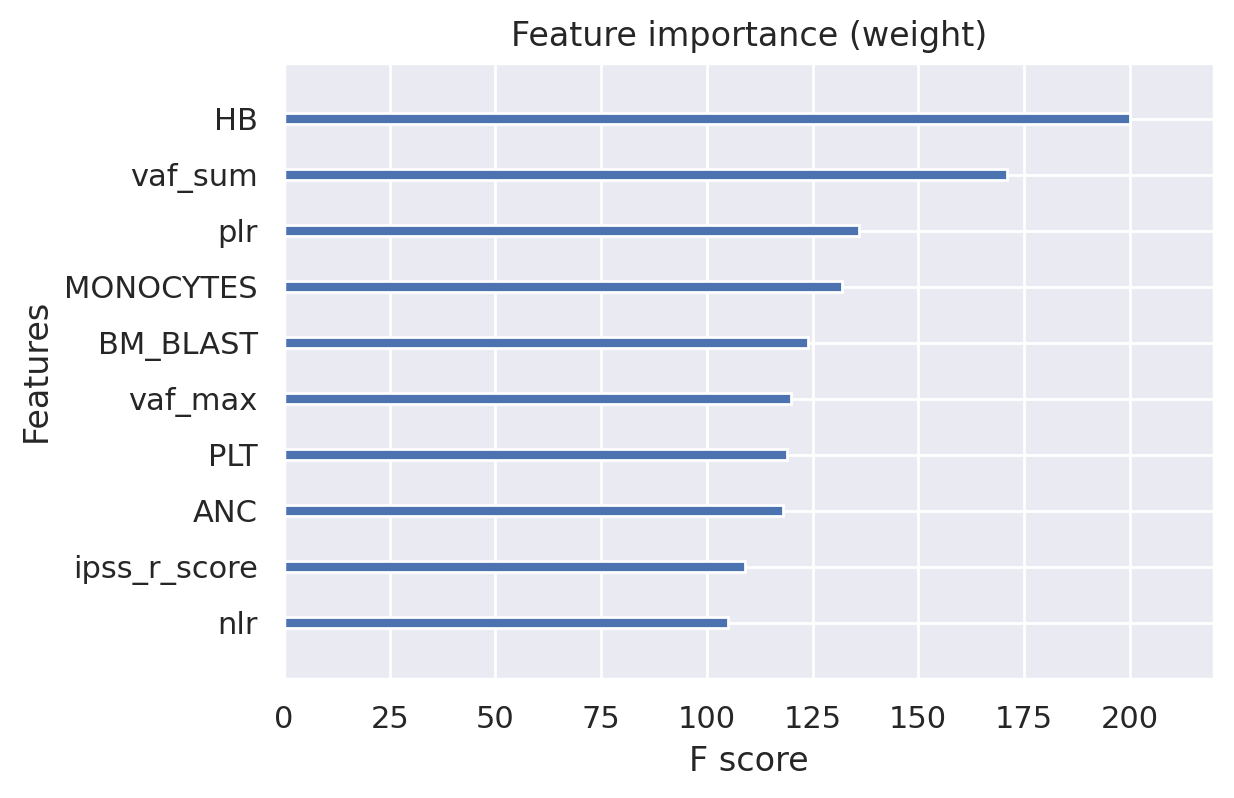
\includegraphics[width=0.6\textwidth]{img/feature_importance_xgb_weight.png}
    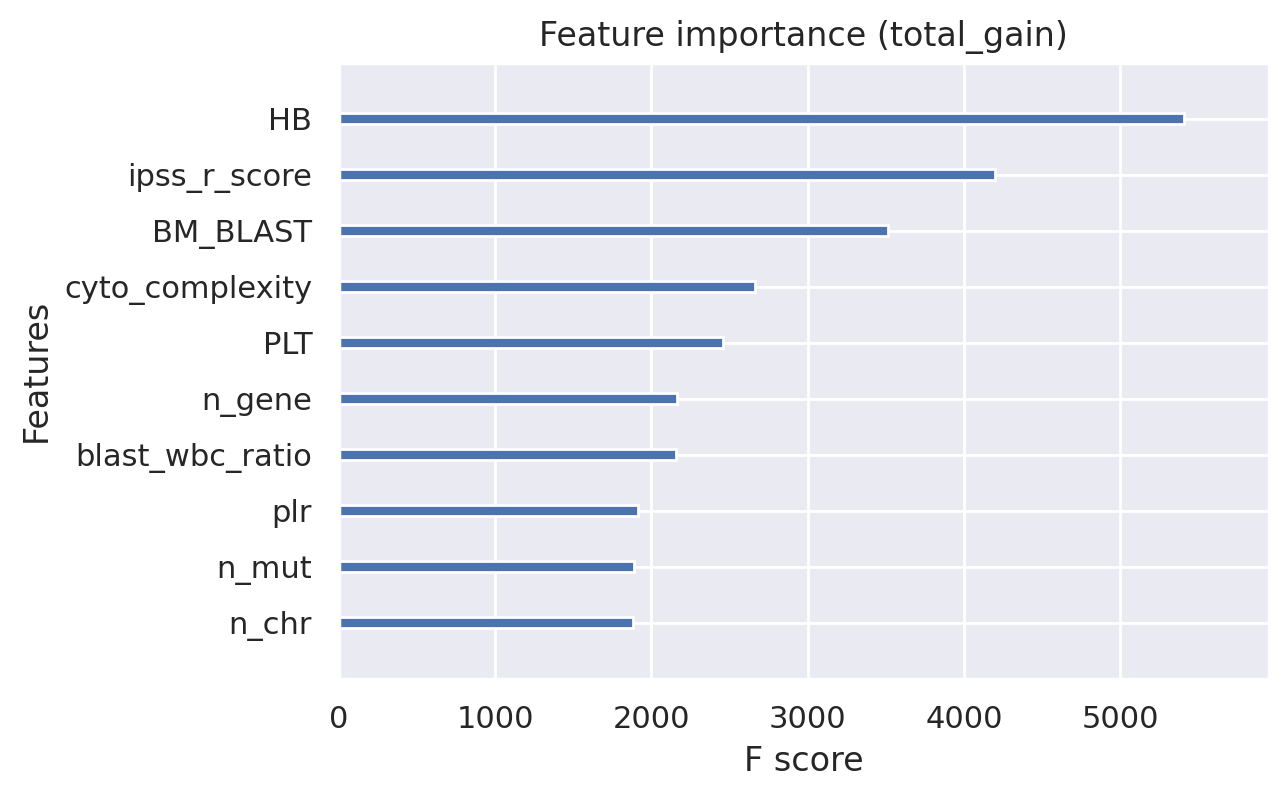
\includegraphics[width=0.6\textwidth]{img/feature_importance_xgb_total_gain.png}
    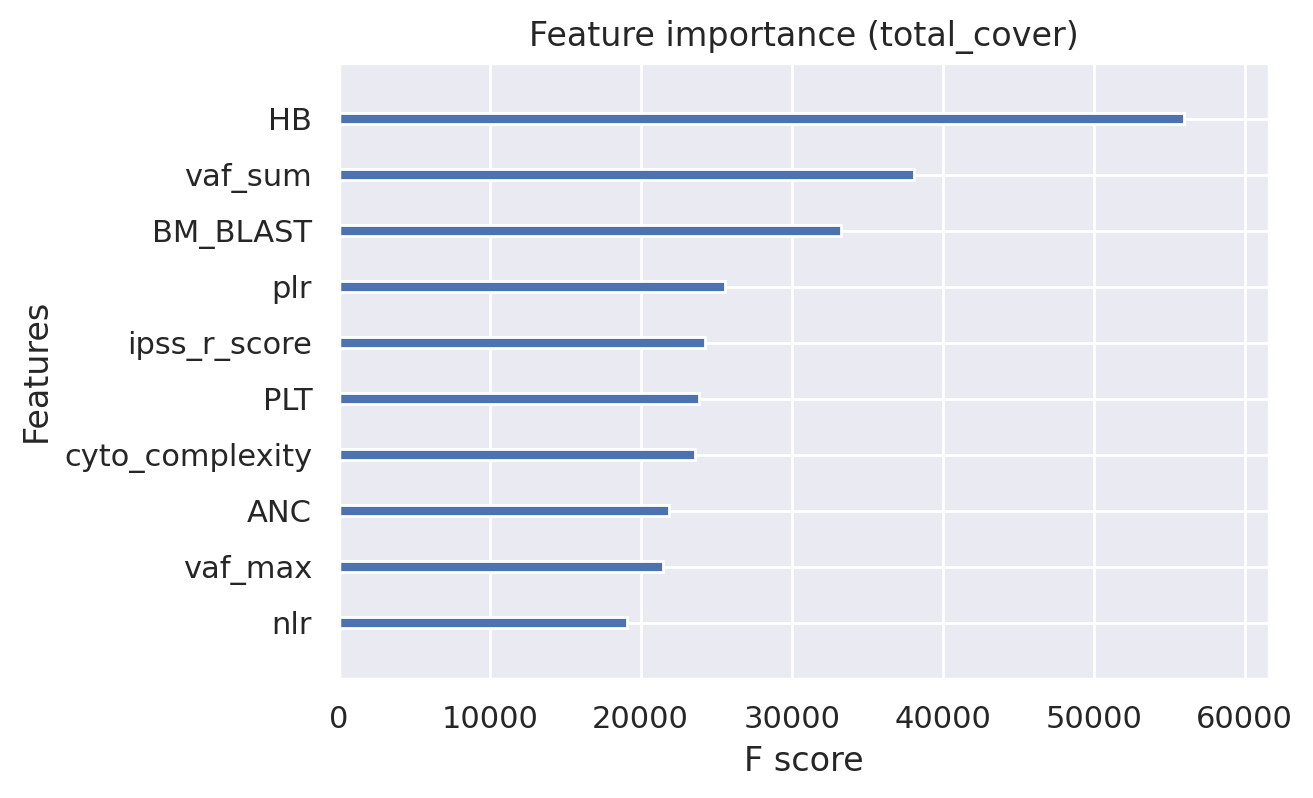
\includegraphics[width=0.6\textwidth]{img/feature_importance_xgb_total_cover.png}
    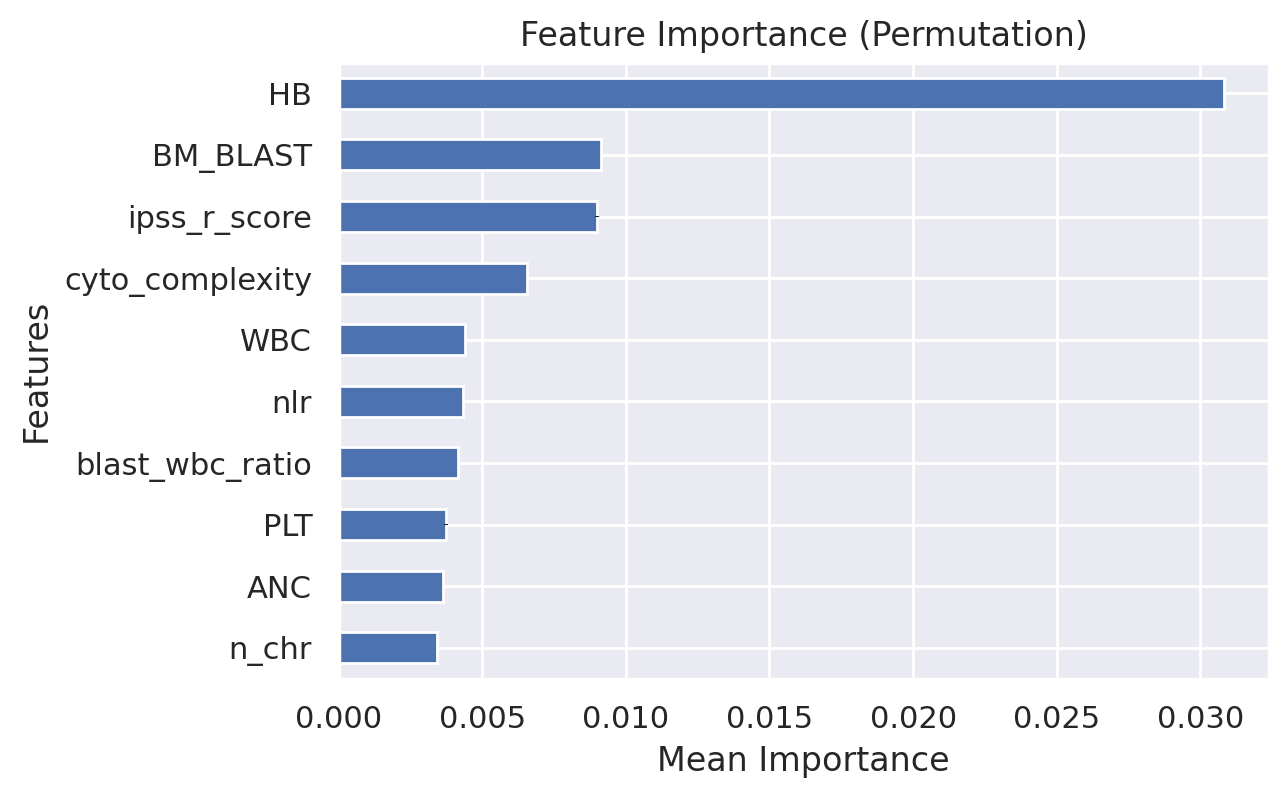
\includegraphics[width=0.6\textwidth]{img/feature_importance_xgb_permutation.png}
    \caption{Feature importance scores for XGBoost model.}
    \label{fig:feature_importance}
\end{figure}


\subsection{Analysis of model performance}

The analysis of our model performance is not straightforward because the IPCW-C-index is complex. Since we are trying to predict the (relative) risk score of patients, one natural way to analyze the performance of our model is to look at how informative the risk score is. We can view this question using notions from classification, as if we were trying to predict whether the patient will die within the next 7 years\footnote{We censored observations at 7 years to compute C-IPCW.} or not. We can thus define the following notions:
\begin{itemize}
    \item \textbf{Precision}: When our model flags a patient as high-risk (resp. low-risk) does the patient indeed die within 7 years (resp. not die within 7 years)?
    \item \textbf{Recall}: When a patient dies (resp. doesn't die) within 7 years, does our model flag them as high-risk (resp. low-risk)?
    \item What happens for mid-risk patients?
\end{itemize}

To answer these questions, we can look at the scatter plot of the risk score against the actual survival time and survival class. The results are shown in Figure \ref{fig:precision_recall}. We find that the model has \textit{good precision for low-risk patients} (blue oval) and \textit{high precision for high-risk patients} (yellow oval). However, the model has \textit{medium recall for high-risk patients} (purple oval). Finally, the model is globally \textit{uncertain for mid-risk patients} (green oval). This is not surprising as the model is trying to predict a continuous variable (the risk score) and the outcome is binary (death of not).

To summarize our analysis: our model is good at flagging low-risk patients and high-risk patients, but it is moderately good at catching high-risk patients. Besides, our model globally behaves poorly outside the extremes: that is, our risk score is not very informative for mid-risk patients.

\begin{figure}[htbp!]
    \centering
    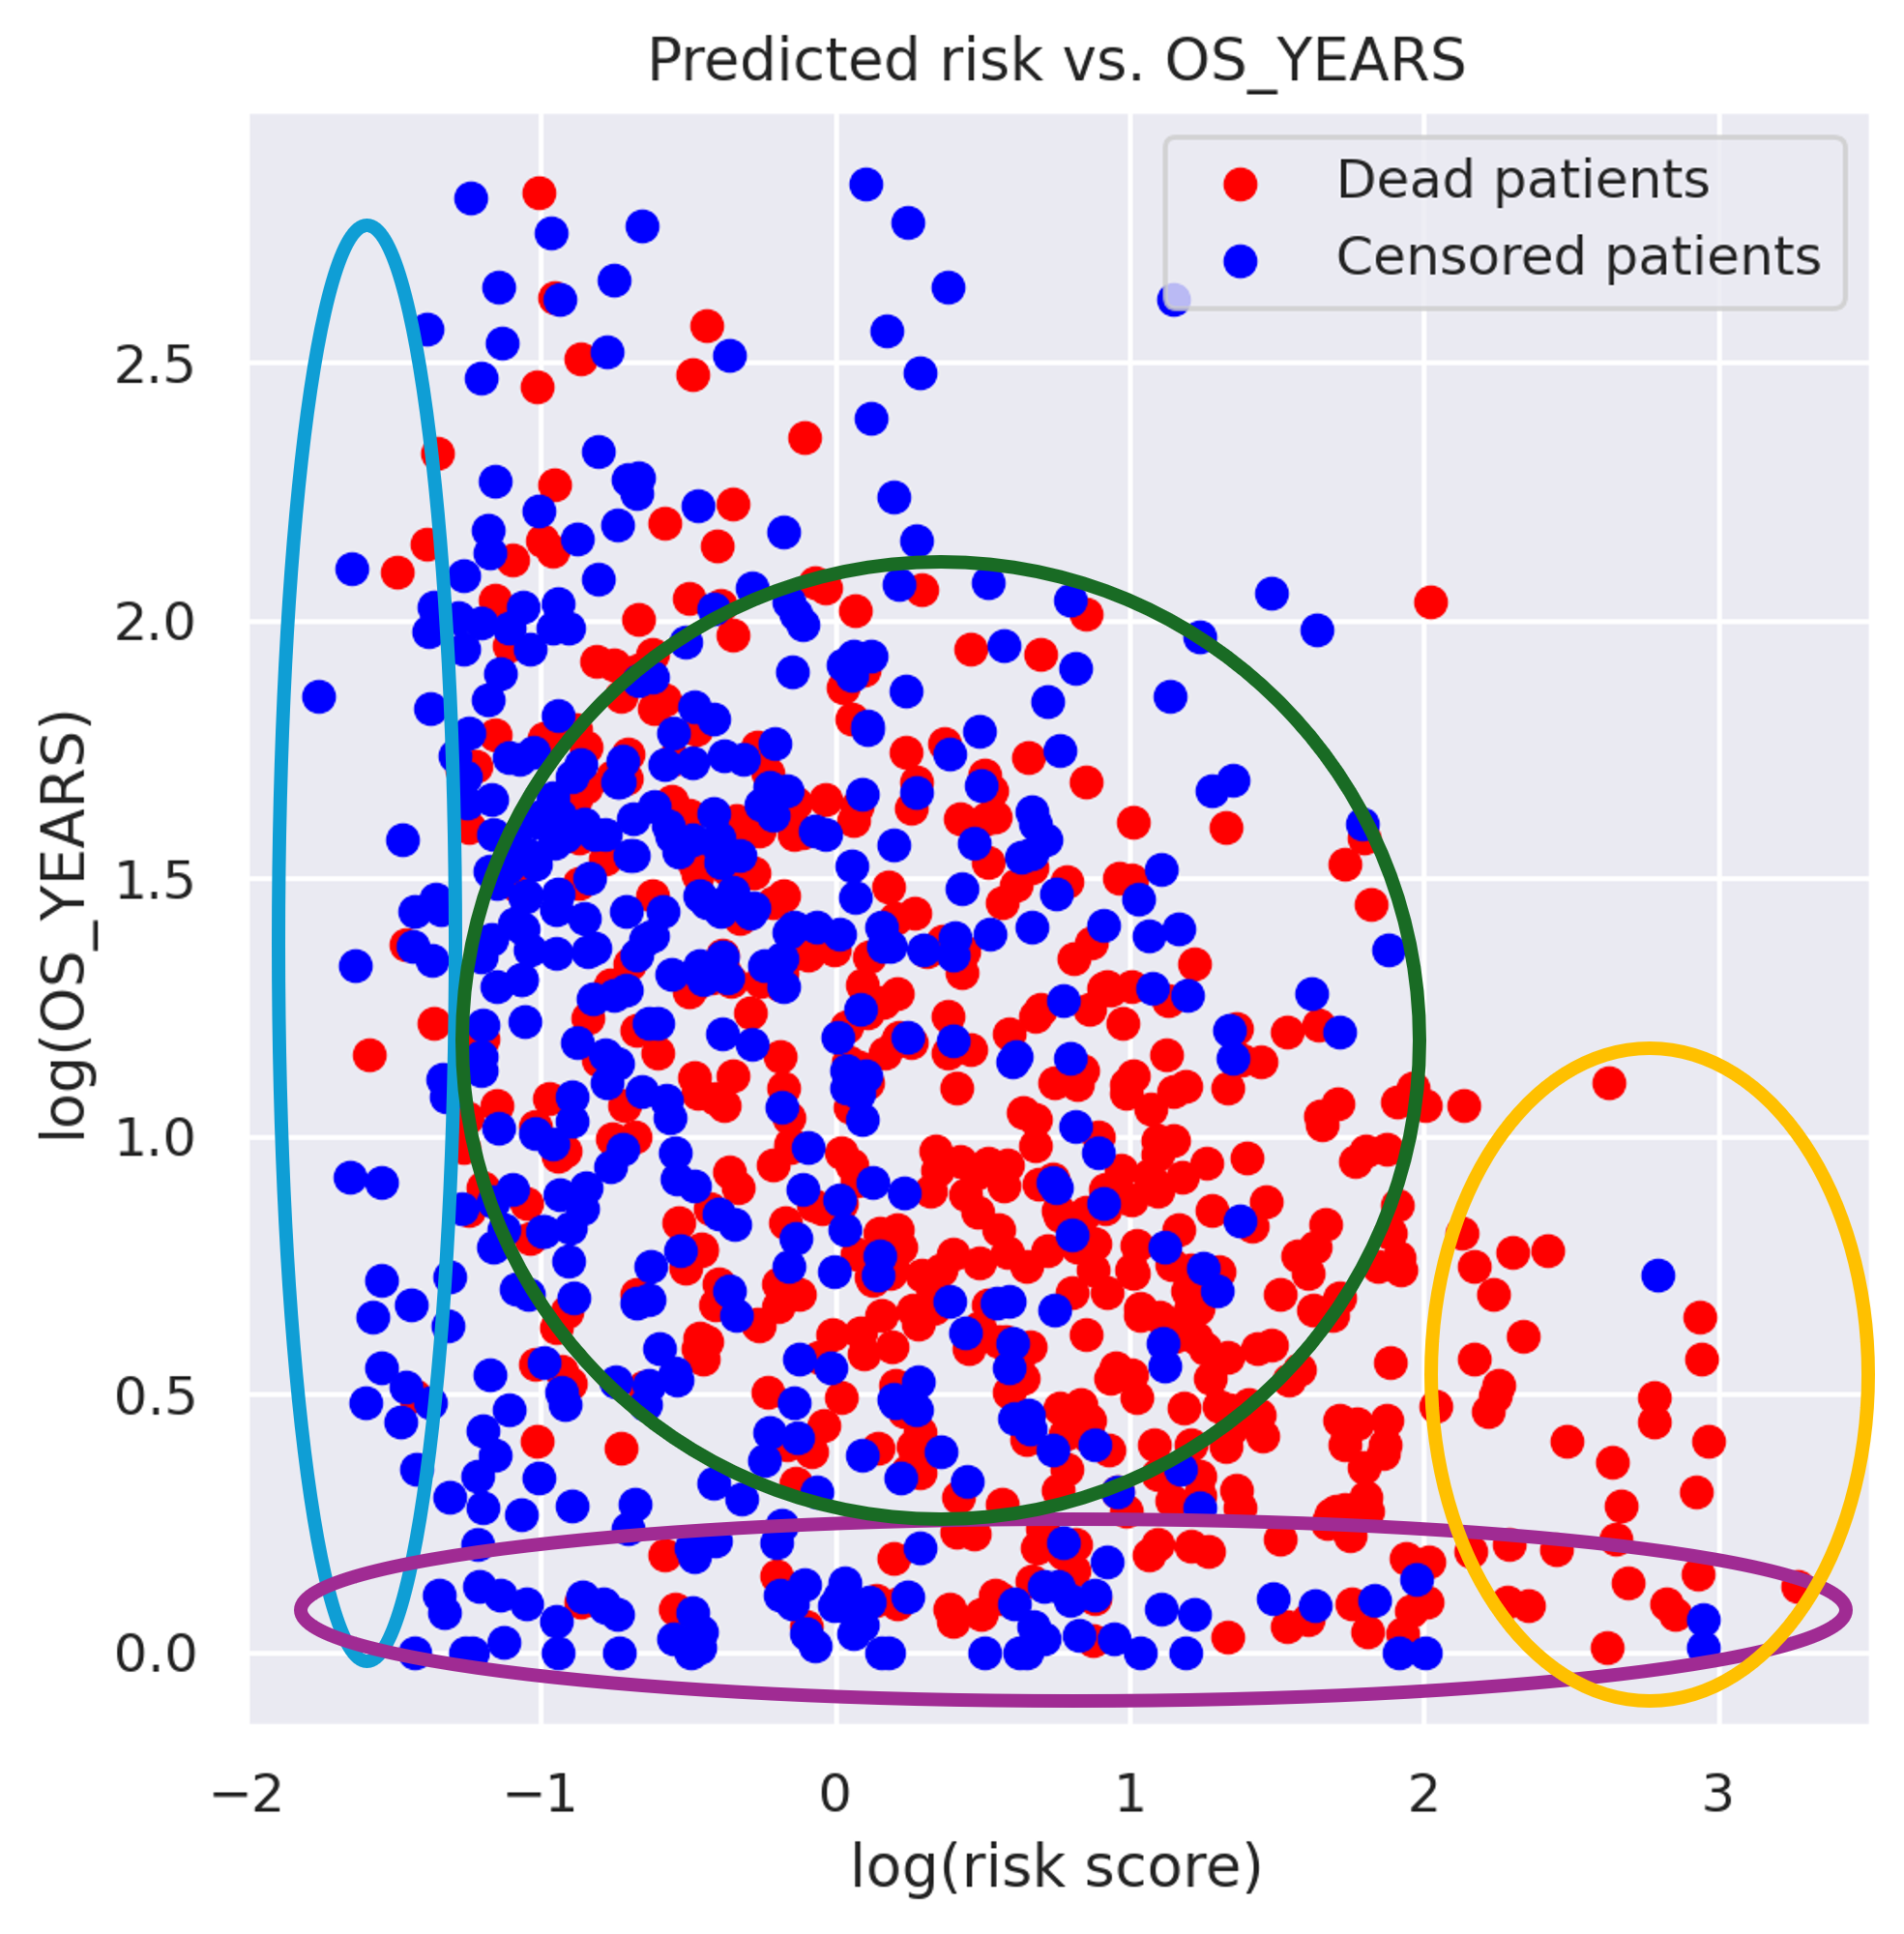
\includegraphics[width=0.8\textwidth]{img/risk_score_vs_OS_YEARS_annotated.png}
    \caption{Scatter plot of risk score against actual survival time, colored by survival class.}
    \label{fig:precision_recall}
\end{figure}

\section{Conclusion and Future Work}
While XGBoost performs well at flagging high and low-risk patients, intermediate-risk predictions remain uncertain, and recall is medium on high-risk patients. This suggests that the model is not very informative for mid-risk patients, which is a significant limitation.

Several approaches can be explored to improve our model's performance:
\begin{itemize}
    \item \textbf{Feature Engineering}: We could leverage medical literature on AML to create more informative features, especially for genetic data and cytogenetics. For example, we could create very specific features based on the presence of specific mutations or chromosomal abnormalities that are known to be associated with poor prognosis.
    \item \textbf{Ensembling}: Combining different models would almost certainly improve performance and robustness, but it is nontrivial since we first need to somehow make the risk scores comparable. We could also simply use a stacking metamodel to combine the predictions of different models without needing to make the risk scores comparable, but then the risk of overfit is very high, so we would probably need to use a very simple model as a metamodel, or gather more data...
    \item \textbf{Hyperparameter Tuning}: Further tuning of hyperparameters could yield better performance, especially for the XGBoost model. However we run the risk of overfitting the data, so we should be careful and use a validation set to evaluate the performance of the model.
    \item \textbf{Model Selection}: Exploring other models could lead to better performance, for instance deep learning models, which are known to perform well on high-dimensional data. However, they are also more prone to overfitting and require more data to train properly.
    \item \textbf{More Data}: Gathering more data could help improve the model's performance. This could be done by collaborating with other hospitals or institutions to gather more data on AML patients.
\end{itemize}
 

\begin{thebibliography}{9}

    \bibitem{AML Risk Factors}
    Pourrajab F, Zare-Khormizi MR, Hashemi AS, Hekmatimoghaddam S. Genetic Characterization and Risk Stratification of Acute Myeloid Leukemia. Cancer Manag Res. 2020 Mar 25;12:2231-2253. doi: 10.2147/CMAR.S242479. PMID: 32273762; PMCID: PMC7104087.
    \url{https://pubmed.ncbi.nlm.nih.gov/32273762/}

    \bibitem{IPSS-R}  
    Revised international prognostic scoring system for myelodysplastic syndromes. Blood. 2012 Sep 20;120(12):2454-65. doi: 10.1182/blood-2012-03-420489. Epub 2012 Jun 27. PMID: 22740453; PMCID: PMC4425443.
    \url{https://pubmed.ncbi.nlm.nih.gov/22740453/}

    \bibitem{scikit-survival}
    Scikit-survival: A library for survival analysis in Python.
    \url{https://scikit-survival.readthedocs.io/en/stable/}
    
    \bibitem{XGBoost}
    XGBoost: A scalable tree boosting system.
    \url{https://xgboost.readthedocs.io/en/latest/}

    \bibitem{optuna}
    Optuna: A Bayesian hyperparameter optimization framework.
    \url{https://optuna.org/}
\end{thebibliography}

\end{document}
